% Template for Cogsci submission with R Markdown

% Stuff changed from original Markdown PLOS Template
\documentclass[10pt, letterpaper]{article}

\usepackage{cogsci}
\usepackage{pslatex}
\usepackage{float}
\usepackage{caption}

% amsmath package, useful for mathematical formulas
\usepackage{amsmath}

% amssymb package, useful for mathematical symbols
\usepackage{amssymb}

% hyperref package, useful for hyperlinks
\usepackage{hyperref}

% graphicx package, useful for including eps and pdf graphics
% include graphics with the command \includegraphics
\usepackage{graphicx}

% Sweave(-like)
\usepackage{fancyvrb}
\DefineVerbatimEnvironment{Sinput}{Verbatim}{fontshape=sl}
\DefineVerbatimEnvironment{Soutput}{Verbatim}{}
\DefineVerbatimEnvironment{Scode}{Verbatim}{fontshape=sl}
\newenvironment{Schunk}{}{}
\DefineVerbatimEnvironment{Code}{Verbatim}{}
\DefineVerbatimEnvironment{CodeInput}{Verbatim}{fontshape=sl}
\DefineVerbatimEnvironment{CodeOutput}{Verbatim}{}
\newenvironment{CodeChunk}{}{}

% cite package, to clean up citations in the main text. Do not remove.
\usepackage{apacite}

% KM added 1/4/18 to allow control of blind submission


\usepackage{color}

% Use doublespacing - comment out for single spacing
%\usepackage{setspace}
%\doublespacing


% % Text layout
% \topmargin 0.0cm
% \oddsidemargin 0.5cm
% \evensidemargin 0.5cm
% \textwidth 16cm
% \textheight 21cm

\title{Child language input does not reflect world frequency: Typical and
atypical feature description across development}


\author{{\large \bf Morton Ann Gernsbacher (MAG@Macc.Wisc.Edu)} \\ Department of Psychology, 1202 W. Johnson Street \\ Madison, WI 53706 USA \AND {\large \bf Sharon J.~Derry (SDJ@Macc.Wisc.Edu)} \\ Department of Educational Psychology, 1025 W. Johnson Street \\ Madison, WI 53706 USA}

\begin{document}

\maketitle

\begin{abstract}
Language provides children a powerful source of information about the
world. From language alone, simple distributional learning models can
recover enough information to perform comparably to non-native college
applicants on the TOEFL (Landauer \& Dumais, 1997). Blind children learn
the same kinds of relationships among perceptual categories as sighted
children, without any of the relevant visual input (Landau \& Gleitman,
1985). However, language does not perfectly reflect the world: the most
typical features of natural kinds may often go unremarked. For instance,
adults rarely describe the color of an orange carrot, as world knowledge
makes this description redundant. Given children's nascent world
knowledge, does parents' speech to children follow this pattern? From
longitudinal corpus data of parent-child communication (Goldin-Meadow et
al., 2014) between 14--58 months, we extracted usage data for 684
high-frequency concrete nouns and co-occurring adjectives. Independent
raters coded the typicality of over 2,000 unique adjective--noun pairs
on a 7-point Likert scale. If language statistics reflect world
statistics, description should be dominated by the typical (strong
negative skew); however, across all ages, we see descriptors
concentrated in the atypical range (positive skewness = 0.65). However,
parents were reliably more likely to use typical descriptors when
talking to younger copmared with older children. Overall, child language
input reflects notable more than typical features, but increased
description of typical features early in development may provide a
foothold for young learners.

\textbf{Keywords:}
language input, language acquisition, child-directed speech
\end{abstract}

Children learn a tremendous amount about the structure of the world
around them in just a few short years, from the rules that govern the
movement of physical objects to the hierarchical structure of natural
categories and even relational structures among social and cultural
groups (Baillargeon, 1994; Legare \& Harris, 2016; Rogers \& McClelland,
2004). Where does the information for this rapid acquisition come from?
Undoubtedly, a sizeable component comes from direct experience observing
and interacting with the world (Sloutsky \& Fisher, 2004; Stahl \&
Feigenson, 2015). But another important source of information comes from
the language people use to talk about the world (Landauer \& Dumais,
1997; Rhodes, Leslie, \& Tworek, 2012).

How similar is the information available from children's direct
experience to the information available in the language children hear?
Several lines of work suggest that they may be surprisingly similar. One
compelling area of work is the comparison of semantic structures learned
by congentinally blind children to those of their sighted peers. In
several domains that would at first blush rely heavily on perceptual
information, such as color terms or verbs of perception (e.g.
\emph{look}, \emph{see}), blind children's semantic similarity judgments
are quite similar to those of sighted children (Landau, Gleitman, \&
Landau, 2009). Further, blind adults' judgments of perceptual verbs are
sensitive to highly detailed information like variation in intensity
(e.g.~blaze vs.~glow), just like sighted adults (Bedny, Koster-Hale,
Elli, Yazzolino, \& Saxe, 2019). Another piece of evidence in favor of
the redundance of vision and language is the broad success of
statistical models trained on language alone in approximating human
judgments across a variety of domains (Landauer \& Dumais, 1997;
Mikolov, Sutskever, Chen, Corrado, \& Dean, 2013, @devlin2018). Language
information, even in isolation, clearly provides sufficient structure to
bootstrap learning across a number of dimensions.

However, a great deal of theoretical claims and experimental work
suggest that language is not a veridical mirror of the world, but is
instead used to selectively comment on the new and the unusual; thus,
language may be argued to contain information that is highly divergent
from world statistics (CITATION). On pragmatic accounts of language,
people typically are `as informative as is required' in their language,
not more or less so (Grice, 1979). Thus, speakers are informative in
relation to common knowledge amongst interlocutors and available
information in the environment, not redundant with these other sources
of knowledge. Language production tasks in the lab largely bolster this
claim, finding that people are sensitive to informativity in formulating
and interpreting utterances (e.g., Rubio-Fernandez, 2016). In
particular, speakers are informative in relation to both the current
context of objects in the environment and the typical features of those
objects (Rubio-Fernandez, 2016). While speakers overwhelmingly refer to
an object that is typical of its category with a bare noun---e.g.,
calling a yellow banana ``a banana''---they often describe more about
the object's features when they are atypical, rarely referring to a
green or blue banana without specifying its color. Listeners are
similarly affected by color description, expecting a color adjective to
be used when an object's color is atypical (Sedivy, 2003).

While such effects have been demonstrated in the lab, the extent to
which these language pressures structure naturalistic language remains
unclear. A recent analysis of co-occuring adjective-noun pairs in the
Wikipedia corpus asked human raters to judge the whether a given
adjective was `always true', `sometimes true', or `never true/unrelated'
to a co-occuring noun (Willits,// \emph{personal communication } // ? ).
The analysis revealed that language usage is dominated by descriptions
that are only `sometimes true' of the described category, and thus
suggests that naturalistic language usage reflects pressures to comment
on the atypical (Willits,// \emph{personal communication } // ? ).

If the information in language statistics is indeed not a reflection of
world statistics, young children may be faced with a difficult learning
problem. Language provides a crucial information source for young
children to learn about the complex world around them (Landauer \&
Dumais, 1997; Rhodes et al., 2012). Without the relevant world
knowledge, young children learning from language input that is biased to
overrepresent atypical features could develop inaccurate or distorted
understandings of the categories being described.

It could be that the language input to young children is far different
from the language on Wikipedia, such that children are learning from
language that is much more veridical than the world around them.
Child-directed speech (CDS) differs from typical adult-directed speech
along a number of structural dimensions, having simpler syntax and more
reduplications (Snow, 1972).CDS also changes across development, with
parents modulating the way they talk as a function of child's age (Snow,
1972). It is plausible that caregivers, especially of young children,
would provide more description of typical features, whether simply to
communicate effectively with a child who has less world knowledge or to
explicitly teach their child about the world. The current study asks
whether CDS is biased to highlight atypical features, as in adult speech
(WILLITS, personal communication), or to more veridically reflects
typical information about the world.

We first asked how information is distributed in CDS, and how similar it
is to ADS. In a longitudinal corpus of parent-child communication, we
collected usage data for adjective-noun pairs that co-occur within the
same utterance. Human raters on Amazon Mechanical Turk then judged
typicality (e.g., ``How common is it for a banana to be a yellow
banana?'') on a 7-point scale. Using these data, we first demonstrate
that child-directed speech (even to children as young as 14 months) is
dominated by descriptions of lower-typicality features (e.g., ``green
banana''), rather than potentially redundant highly-typical features
(e.g., ``yellow banana'').

We next asked if the kind of information in CDS changes as children
develop. We find evidence that description changes across development,
with young children hearing relatively more talk about highly-typical
features compared with older children.

We lastly discuss what these data may imply for the developing learner.
Children rapidly develop sophisticated conceptual repetoires, yet the
language children hear seems biased to overrepresent certain features.
We consider a few potential cues that could allow children to extract
better typicality information from language, such as tracking
second-order co-occurence or possible syntactic cues.

\hypertarget{corpus-analysis}{%
\section{Corpus Analysis}\label{corpus-analysis}}

We first analyze caregiver speech to extract the usage statistics for
all co-occuring adjective-noun pairs within an utterance. After
subsetting the data to the concrete concepts (Brysbaert et al., 2014),
human raters judged the typicality of each adjective-noun pair.
Combining our usage data across the developmental range (ages 14-58
months) with the typicality judgements, we can examine how information
is distrubted in caregiver descriptions.

\hypertarget{corpus-method}{%
\subsubsection{Corpus Method}\label{corpus-method}}

We used data from the Language Development Project-- a large-scale,
longitudinal corpus of parent child-interaction in the home with
families who are representative of the Chicago community in
socio-economic and racial diversity (Goldin-Meadow et al., 2014).
Recordings were taken in the home every 4-months from when the child was
14-months-old until they were 58-months-old, resulting in 12 timepoints.
Recordings were 90 minute sessions, and participants were given no
instructions. The Language Development Project corpus contains
transcription of all speech and communicative gestures produced by
children and their caregivers over the course of the 90-minute home
recordings.

To determine the extant information structure in children's language
input, we subset the corpus to only caregiver speech, yielding a set of
828,392 distinct utterances. While it is important to consider
children's own productions as an integral part their language
environments (CITATION), description of a concept relies heavily on
linguisitic and world knowledge, and so it is necessary to analyze
caregiver speech separately. For example, at our earliest timepoint
(14-months), children are not producing multiword utterances with
adjectives and nouns, or even reliably producing many adjectives at all.

Based on part-of-speech tags, we extracted usage rates for all nouns in
the corpus. To ensure that the set of nouns we examined were relatively
constant across our developmental samples, we subset all nouns that
caregivers produced to only include nouns that were produced at least
once every 3 sessions (i.e.~per developmental year). This yielded a set
of some 2,000 potential target nouns.

We next tagged every utterance that included both one of the target
nouns and an adjecitve. Any possible resulting pairs was counted
seperately (i.e.~utterances with one noun and multiple adjectives were
coded as multiple pairs ) Many resulting high-frequency pairs proved
difficult to classify on our typicality schema (e.g., ``good''--
``job''; ``little'' -- ``bit''). To identify potentially problematic
pairs, we joined human judgments of concreteness for both the noun and
the adjective (Brysbaert). We set our threshold at the top 25\% of the
concreteness ratings, and excluded any pair where either the adjective
or noun was not rated above that threshold. Finally, all pairs were
given to 7 human coders to judge whether the pair was ``incoherent or
unrelated'' and we thus excluded a further XXX pairs from the sample
(e.g., incoherent pairs such as ``wet'' -- ``brown'', and presumably
errorfully coded pairs such as ``orange'' -- ``orange'').

Thus, our final sample included 2,220 unique adjective-noun pairs drawn
from over 6,000 utterances. The pairs were combinations of 684 distinct
concrete nouns and 118 distinct concrete adjectives. We compiled these
pairs and collected human judgments on Amazon Mechanical Turk for each
pair, as described below. Table 1 contains example utterances from the
final set and typicality judgments from our human raters.

\hypertarget{ratings-method}{%
\subsection{Ratings Method}\label{ratings-method}}

To evaluate the typicality of the adjective--noun pairs pulled from the
corpus, we asked participants on Amazon Mechanical Turk to rate each
pair. Participants were presented with a question of the form ``How
common is it for a cow to be a brown cow?'' and asked to provide a
rating on a seven-point scale: (1) never, (2) rarely, (3) sometimes, (4)
about half the time, (5) often, (6) almost always, (7) always. Each
participant rated 20 pairs, and each pair was rated by four
participants; we used Dallinger {[}CITE{]}, a tool for automating
complex recruitment on Amazon Mechanical Turk, to balance recruitment.
Overall, we recruited 444 participants to rate 2200 adjective--noun
pairs. After exclusions using an attention check, we retained 8580
judgments, with each adjective--noun pair retaining at least two
judgments.

\begin{table}[tb]
\centering
\begin{tabular}{llr}
  \hline
utterance & pair & typicality \\ 
  \hline
especially with wooden shoes & wooden shoe & 2.75 \\ 
  some of our green bananas too & green banana & 3.75 \\ 
  are bananas yellow? & yellow banana & 5.75 \\ 
   \hline
\end{tabular}
\end{table}

\begin{CodeChunk}
\begin{figure}[tb]

{\centering 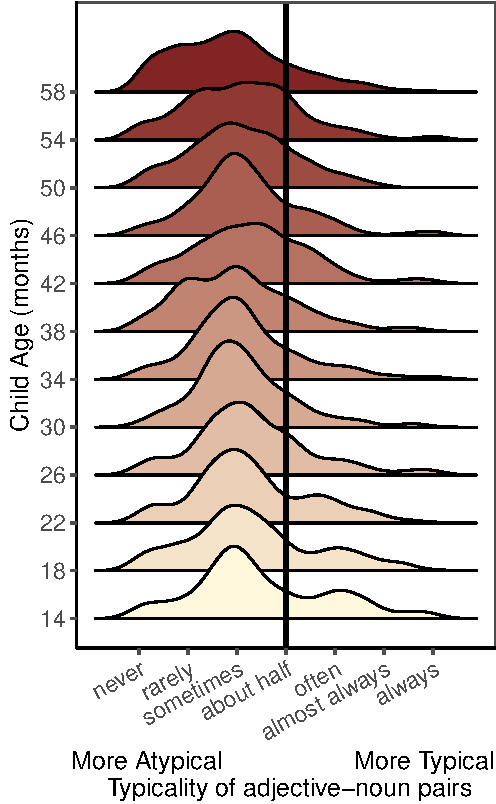
\includegraphics{figs/distribution_plot-1} 

}

\caption[Denisity plots showing the usage amount at each timepoint based on the typicality of the adj-noun pair]{Denisity plots showing the usage amount at each timepoint based on the typicality of the adj-noun pair.}\label{fig:distribution_plot}
\end{figure}
\end{CodeChunk}

\hypertarget{results}{%
\subsection{Results}\label{results}}

If description in child-directed speech mirrors adult-directed speech,
we should see that caregiver descripiton is dominated by modifiers that
are sometimes true of the noun they modify. If instead child-directed
speech privledges redundant or assumed information, caregiver
description would yield a distinct distribution dominated by highly
typical modifiers. As can be seen in figure \ref{fig:distribution_plot},
there is remarkable developmental consistency such that caregiver
description largely focuses on features that are only sometimes true of
the concept.

\hypertarget{developmental-consistency.}{%
\subsubsection{Developmental
Consistency.}\label{developmental-consistency.}}

Examining usage data as a function of typicality (see figure
\ref{fig:distribution_plot}), we see evidence of a positive skew (0.65)
such that the bulk of language reflects adjective-noun pairs rated
\textless{} 4 on typicality (i.e. `sometimes', `rarely' or `never').
Data from every time point from 14-58 months seems to show a similar
pattern (skews 0.23 - 0.82). These data suggest that even when talking
with very young children, caregiver speech structures information
similarly to adult-directed speech.

\hypertarget{talk-about-the-highly-typical.}{%
\subsubsection{Talk about the
Highly-Typical.}\label{talk-about-the-highly-typical.}}

Despite of the striking consistency of description in caregiver speech
across development, we were interested in identifying observable
differences in description across development. One such hypothesis was
that the youngest children should be most likely to hear description of
highly typical features, compared to older children. This would suggest
children with the least developed world knowledge actually get more
information about aspects of the world that are likely to be true and
easily learned via observation, compared with older children. Indeed,
when we look at the proportion of all description that is about
highly-typical features (i.e.~features that are `often', `almost
always', or `always' true), we see a significant negative correlation
with age (\emph{r} = -0.8231762, p \textless{} 0.01). While children at
all ages hear more talk about what is atypically true (figure
\ref{fig:distribution_plot}), younger children hear relatively more talk
about what is typically true than older children (figure
\ref{fig:prototypical_plot}, see also figure \ref{fig:mean_change}).

\begin{CodeChunk}
\begin{figure}[tb]

{\centering 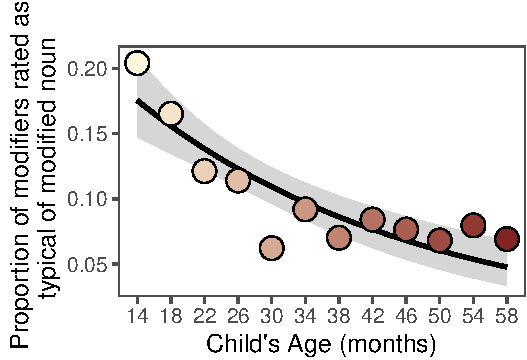
\includegraphics{figs/prototypical_plot-1} 

}

\caption[This plot shows the proportion of caregiver description that is about typically-true features, as a function of age]{This plot shows the proportion of caregiver description that is about typically-true features, as a function of age.}\label{fig:prototypical_plot}
\end{figure}
\end{CodeChunk}

\hypertarget{other-ways-of-extracting-structure-from-language}{%
\section{Other Ways of Extracting Structure from
Language?}\label{other-ways-of-extracting-structure-from-language}}

\hypertarget{second-order-co-occurence}{%
\subsection{Second-order Co-occurence}\label{second-order-co-occurence}}

In our analyses of the concrete adjectives parents use to describe
concrete nouns to their children, we find that parents tend to describe
atypical rather than typical features of objects. This usage aligns with
the idea that language is used informatively in relation to background
knowledge about the world. It may pose a problem, however, for young
language learners with still-developing world knowledge. If language
does not transparently convey the typical features of objects, and
instead (perhaps misleadingly) notes the atypical ones, how might one
use language to learn what objects are typically like? One possibility
is that information about typical features is captured in regularities
across many utterances.

Kim et al. (2019) demonstrate blind people's striking convergence with
sighted people's feature judgments about animals, and posit that blind
people may use animal taxonomy knowledge to selectively generalize
features between species. In a response, Lewis et al. (2019) note that
complex inferential machinery is not necessary to make these nuanced
generalizations, and in fact much of this feature information is
captured by simpler associations between words in the language one
hears. We take a similar approach to ask whether typical feature
information is expressed in the structure of the language children hear.

Information in language goes beyond what can be learned from any one
utterance. Though one might never hear the words /kumquat/ and
/grapefruit/ in the same sentence, their common contexts---other words
like /eat/, /rind/, /tree/, /tart/, and /seeds/---are clues that they
have some similarities. Models of distributional semantics capitalize on
these patterns by representing words using their contexts, and judging
two words to be similar if they are surrounded by similar sets of words.
Though we found that children get more information about atypical than
typical features of objects on the utterance level, perhaps patterns of
language use across many utterances could be used to extract typical
feature information.

\hypertarget{word2vec}{%
\subsubsection{Word2Vec}\label{word2vec}}

To test this possibility, we trained word2vec, a model that predicts
words using their contexts, on the same corpus of child-directed speech
used in our first set of analyses. Our model is a
continuous-bag-of-words word2vec model trained using the package gensim
{[}CITE{]}. If the model captures information about the typical features
of objects, we should see that the model's word pair similarities are
correlated with the typicality ratings we elicited from human raters.

\hypertarget{results-1}{%
\subsubsection{Results}\label{results-1}}

We find that similarities in the model have near zero correlation with
human adjective--noun typicality ratings (r = 0.018). This is in spite
of better correlations with large sets of human similarity judgments
between different kinds of word pairs (correlation with wordsim353,
0.37; correlation with simlex, 0.15). This suggests that statistical
patterns in child-directed speech are likely insufficient to encode
information about the typical features of objects, despite encoding at
least some information about word meaning more broadly. However, the
corpus on which we trained this model was small; perhaps our model did
not get enough language to draw out the patterns that would reflect the
typical features of objects. To test this possibility, we asked whether
word vectors trained on a much larger corpus---English
Wikipedia---strongly correlate with typicality ratings. We find that
while the correlation between similarities in the Wikipedia--trained
model and human noun--adjective typicality ratings is stronger, it is
still fairly weak at r = 0.24. Overall, these results suggest that
models of distributional semantics fail to extract typical feature
information from language in which atypical features are more often
described.

\begin{CodeChunk}
\begin{figure}[tb]

{\centering 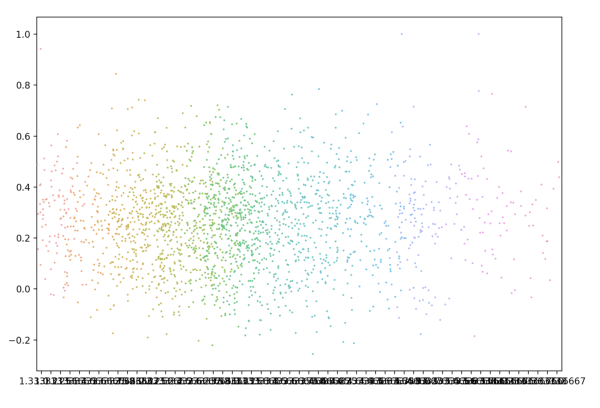
\includegraphics{figs/word2vec-1} 

}

\caption[Correlation of vector distances from word2vec (trained on the LDP corpus) and human-rated typicality judgments]{Correlation of vector distances from word2vec (trained on the LDP corpus) and human-rated typicality judgments.}\label{fig:word2vec}
\end{figure}
\end{CodeChunk}

\hypertarget{age-of-aquisition}{%
\subsection{Age of Aquisition}\label{age-of-aquisition}}

Given our finding that young children hear relatively more description
of typical features, it could be that linguistic input is more helpfully
structured for the developing learner if we have a more nuanced measure
linguistic experience. For example, one possibility is that caregivers
are selectively overdescribing (or at least describing typical features)
of concepts unfamiliar to their child. This possibility makes a clear
prediction: namely, that information in CDS to children at a given age
may differ as a function of whether the child knows the word being
described, or not.

To address this question we combined age of aquisition data from
Wordbank and from adult-generated recollections (Kuperman et al., 2012).

\hypertarget{syntax}{%
\subsection{Syntax}\label{syntax}}

\hypertarget{other-pieces-to-include}{%
\section{Other pieces to include?}\label{other-pieces-to-include}}

\hypertarget{child-productions}{%
\section{Child Productions}\label{child-productions}}

What kind of information is contained in children's own speech? By
analyzing at children's productions, we can determine when children come
to use description in a way that looks like caregiver speech. Are
children mirroring adult-like uses of description even from a young age,
or are they choosing to describe other features of the world?

\hypertarget{method.}{%
\subsubsection{Method.}\label{method.}}

The Language Development Corpus contains 442,048 child utterances. Using
the same data-processing pipeline described for the caregiver speech, we
filter to utterances which contain both at least one adjective and at
least one noun and filter to include only concrete concepts (Brysbaert
et al., 2014). Using the set of adjective-noun pairs for which we have
judgments from our analysis of caregiver speech, we end up with a set of
533 distinct adjective-noun pairs. Note that at our earliest timepoints
(14 and 18 months), children were not reliably producing enough
utterances with adjectives and nouns to be included.

\hypertarget{results.}{%
\subsubsection{Results.}\label{results.}}

Examining usage data as a function of typicality (see figure
\ref{fig:kid_plot}), we again see evidence of a positive skew (0.61,
comapre with skewness = 0.65 seen in the adults), such that the bulk of
language reflects adjective-noun pairs rated \textless{} 4 on typicality
(i.e. `sometimes', `rarely' or `never'). A t-test confirms that
children's description focuses on the atypical (mean typicality = 3.2)
rather than the typical (compared with a null-value of 4 or ``about
half'') (\emph{t} = -25.44, p\textless{}0.001).

These data suggest that children's productions, like adults, focus on
describing less typical features of world. Of course, these utterances
come from naturalistic conversations with caregivers, and the pattern of
description is likely highly dependent on the interlocutor. That is, if
a parent chooses to describe the \emph{purpleness} of a cat in book, the
child may well respond by asking about that same feature. Thus it is
perhaps unsurpising that their usage patterns would be well-aligned.

\begin{CodeChunk}
\begin{figure}[tb]

{\centering 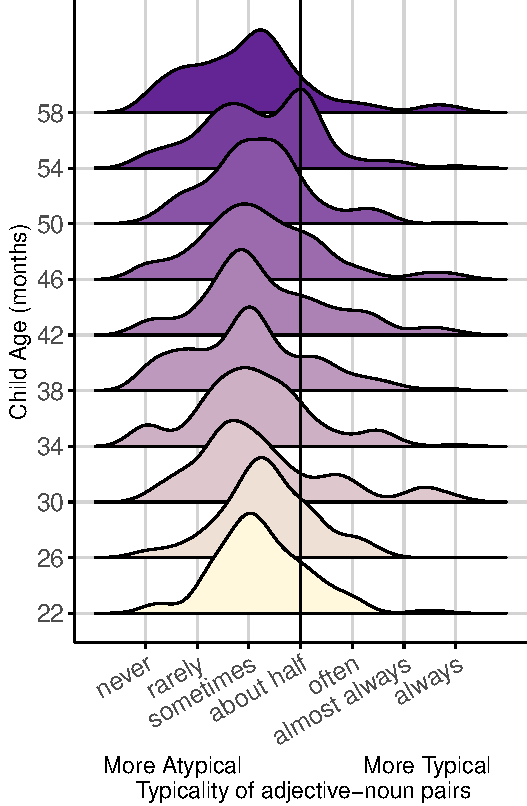
\includegraphics{figs/kid_plot-1} 

}

\caption[Analyzing child productions, these denisity plots show the usage amount at each timepoint based on the typicality of the adj-noun pair]{Analyzing child productions, these denisity plots show the usage amount at each timepoint based on the typicality of the adj-noun pair. Note that at our earliest timepoints (14 and 18 months), children were not reliably producing enough utterances with adjectives and nouns to be included here.}\label{fig:kid_plot}
\end{figure}
\end{CodeChunk}

\hypertarget{adult-comparison}{%
\section{Adult Comparison}\label{adult-comparison}}

To understand a reasonable hile some recent work has established a
general pattern of

\hypertarget{method.-1}{%
\subsubsection{Method.}\label{method.-1}}

Examining data from the Corpus of Contemporary American English, we can
look at adult-directed speech across a range of settings. Using the same
data-processing pipeline described for the caregiver speech, we filter
to utterances which contain both at least one adjective and at least one
noun and filter to include only concrete concepts (Brysbaert et al.,
2014). Using the set of adjective-noun pairs for which we have judgments
from our analysis of caregiver speech, we end up with a set of 1,357
distinct adjective-noun pairs.

\hypertarget{results.-1}{%
\subsubsection{Results.}\label{results.-1}}

Examining usage data as a function of typicality (see figure
\ref{fig:adult_directed}), we again see evidence of a positive skew
(0.68), such that the bulk of language reflects adjective-noun pairs
rated \textless{} 4 on typicality (i.e. `sometimes', `rarely' or
`never'). A t-test confirms that description in adult-directed speech
focuses on the atypical (mean typicality = 3.48) rather than the typical
(compared with a null-value of 4 or ``about half'') (\emph{t} = -211.44,
p\textless{}0.001).

Overall, the usage distributions in adult-directed speech seem
qualitatively similar to the distributions we found in child-directed
speech. The difference of settings makes it difficult to compare these
data directly with our data from the Language Devleopment Project
corpus. Four of the COCA datasets are drawn from written texts, which
puts in place distinct language pressures and removes visual common
ground. While there is one subset of the corpus drawn from spoken data,
those utterances come from TV and radio programs. All of these settings
are likely quite different environements for language than the
naturalistic in-home setting that our Language Development Project
corpus draws from. In light of these differences, any observed
similarity in usage seems remarkable.

\begin{CodeChunk}
\begin{figure}[tb]

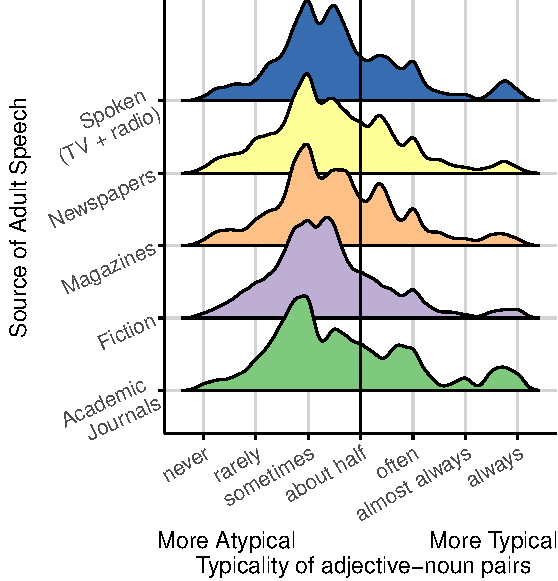
\includegraphics{figs/adult_directed-1} \hfill{}

\caption[Looking at COCA data, these denisity plots show the usage amount based on the typicality of the adj-noun pair, seperated by the type of language (e.g., written)]{Looking at COCA data, these denisity plots show the usage amount based on the typicality of the adj-noun pair, seperated by the type of language (e.g., written).}\label{fig:adult_directed}
\end{figure}
\end{CodeChunk}

\hypertarget{discussion}{%
\section{Discussion}\label{discussion}}

importance of conversational pressures in determining information in
language

\begin{quote}
AL: ``Why would adults provide so little typical feature information (or
at least less than we might think)? Are they just avoiding
over-informativity, even with presumably more ignorant conversational
partners? Maybe the way they talk is actually important for kids to
learn pragmatics / how to talk about features?''
\end{quote}

learning problem for kids. maybe the prototypicals is a foothold for
young learners\ldots{}.

\begin{quote}
AL: Do you think there is enough of the prototypicals? given that even
the youngest kids only hear like 20\% typical adjectives -- but maybe
that's already a lot (?)
\end{quote}

more thoughts on potential ways kids extract more information

limitations\ldots{} abstract language?

\hypertarget{acknowledgements}{%
\section{Acknowledgements}\label{acknowledgements}}

Place acknowledgments (including funding information) in a section at
the end of the paper.

\hypertarget{references}{%
\section{References}\label{references}}

\setlength{\parindent}{-0.1in} 
\setlength{\leftskip}{0.125in}

\noindent

\hypertarget{refs}{}
\leavevmode\hypertarget{ref-baillargeon1994}{}%
Baillargeon, R. (1994). How do infants learn about the physical world?
\emph{Current Directions in Psychological Science}, \emph{3}(5),
133--140.

\leavevmode\hypertarget{ref-bedny2019}{}%
Bedny, M., Koster-Hale, J., Elli, G., Yazzolino, L., \& Saxe, R. (2019).
There's more to ``sparkle'' than meets the eye: Knowledge of vision and
light verbs among congenitally blind and sighted individuals.
\emph{Cognition}, \emph{189}, 105--115.

\leavevmode\hypertarget{ref-devlin2018}{}%
Devlin, J., Chang, M.-W., Lee, K., \& Toutanova, K. (2018). Bert:
Pre-training of deep bidirectional transformers for language
understanding. \emph{arXiv Preprint arXiv:1810.04805}.

\leavevmode\hypertarget{ref-landau2009}{}%
Landau, B., Gleitman, L. R., \& Landau, B. (2009). \emph{Language and
experience: Evidence from the blind child} (Vol. 8). Harvard University
Press.

\leavevmode\hypertarget{ref-landauer1997}{}%
Landauer, T. K., \& Dumais, S. T. (1997). A solution to plato's problem:
The latent semantic analysis theory of acquisition, induction, and
representation of knowledge. \emph{Psychological Review}, \emph{104}(2),
211.

\leavevmode\hypertarget{ref-legare2016}{}%
Legare, C. H., \& Harris, P. L. (2016). The ontogeny of cultural
learning. \emph{Child Development}, \emph{87}(3), 633--642.

\leavevmode\hypertarget{ref-mikolov2013}{}%
Mikolov, T., Sutskever, I., Chen, K., Corrado, G. S., \& Dean, J.
(2013). Distributed representations of words and phrases and their
compositionality. In \emph{Advances in neural information processing
systems} (pp. 3111--3119).

\leavevmode\hypertarget{ref-rhodes2012}{}%
Rhodes, M., Leslie, S.-J., \& Tworek, C. M. (2012). Cultural
transmission of social essentialism. \emph{Proceedings of the National
Academy of Sciences}, \emph{109}(34), 13526--13531.

\leavevmode\hypertarget{ref-rogers2004}{}%
Rogers, T. T., \& McClelland, J. L. (2004). \emph{Semantic cognition: A
parallel distributed processing approach}. MIT press.

\leavevmode\hypertarget{ref-sloutsky2004}{}%
Sloutsky, V. M., \& Fisher, A. V. (2004). Induction and categorization
in young children: A similarity-based model. \emph{Journal of
Experimental Psychology: General}, \emph{133}(2), 166.

\leavevmode\hypertarget{ref-stahl2015}{}%
Stahl, A. E., \& Feigenson, L. (2015). Observing the unexpected enhances
infants' learning and exploration. \emph{Science}, \emph{348}(6230),
91--94.

\bibliographystyle{apacite}


\end{document}
